\epi{``I am interested in this and hope to do something.''}
{\textit{On adding complex numbers to Go}\\ \textsc{KEN THOMPSON}}

\noindent{}What is Go? From the website \cite{go_web}:
\begin{quote}
The Go programming language is an open source project to make
programmers more productive. Go is expressive, concise, clean, and
efficient. Its concurrency mechanisms make it easy to write programs
that get the most out of multi core and networked machines, while its
novel type system enables flexible and modular program construction. Go
compiles quickly to machine code yet has the convenience of garbage
collection and the power of run-time reflection. It's a fast, statically
typed, compiled language that feels like a dynamically typed,
interpreted language.
\end{quote}

Go is a young language, where 
features are still being added or even \emph{removed}. It 
may be possible that some text is outdated when you
read it. 
Some exercise answers may become incorrect as Go continues
to evolve.
We will do our best to keep this document up to 
date with respect to the latest Go release.
An effort has been made to create ``future proof'' code examples.

The following convention is used throughout this book:
\begin{itemize}
\item Code is displayed in \prog{DejaVu Mono};
\item Keywords are displayed in \key{DejaVu Mono Bold};
\item Comments are displayed in \rem{DejaVu Mono Italic};
\item Extra remarks in the code \coderemark{Are displayed like this};
\item Longer remarks get a number -- \gocircle{1} -- with the explanation following;
\item Line numbers are printed on the right side;
\item Shell examples use a \pr{} as prompt;
\item User entered text in shell examples \texttt{\user{is in bold}}, system responses
are in a \texttt{typewriter font};
\item An emphasized paragraph is indented and has a vertical bar on the
left.
\end{itemize}

\section{Official documentation}
There already is a substantial amount of documentation written about Go.
\gomarginpar{When searching on the internet use the term ``golang'' instead of plain ``go''.}
The Go Tutorial \cite{go_tutorial}, and the Effective Go
document \cite{effective_go}. The
website \url{http://golang.org/doc/} is a very good starting point
for reading up on Go\footnote{\url{http://golang.org/doc/} itself is served by 
a Go program called \prog{go\ doc}.}. Reading these documents is
certainly not required, but is recommended.

Go comes with its own documentation in the form of a program called
\prog{go doc}. 
You can use it yourself to look
in the on-line documentation. For
instance, suppose we want to know more about the package \package{hash}.
We would then give the command \prog{go doc hash}.
How to create your own package documentation
is explained in chapter \ref{chap:packages}.

\section{Origins}
Go has it origins in Inferno \cite{inferno} (which in turn was based
upon Plan 9 \cite{plan9}). Inferno included a language called Limbo
\cite{limbo}. Quoting from the Limbo paper:
\begin{quote}
Limbo is a programming language intended for applications running
distributed systems on small computers. It supports modular programming,
strong type checking at compile- and run-time, \emph{inter process
communication over typed channels}, automatic \emph{garbage collection}, and
simple abstract data types. It is designed for safe execution even on
small machines without hardware memory protection.
\end{quote}
A feature Go inherited from Limbo is channels (see chapter
\ref{chap:channels}). Again from the Limbo documentation.
\begin{quote}
[A channel] is a communication mechanism capable of sending and receiving objects of
the specified type to another agent in the system. Channels may be used
to communicate between local processes; using library procedures, they
may be connected to named destinations. In either case send and receive
operations may be directed to them.
\end{quote}
The channels in Go are easier to use than those in Limbo.
If we dig even deeper in the history of Go we also find references
to ``Newsqueak'' \cite{newsqueak}, which pioneered the use of 
channel communication in a C--like language. Channel
communication isn't unique to these languages, a big non--C--like
language which also uses them is Erlang \cite{erlang}.

\begin{figure}[H]
\caption{Chronology of Go}
\label{fig:chrono-of-go}
\begin{center}
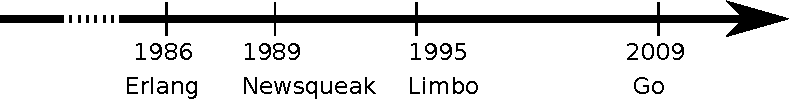
\includegraphics[scale=0.65]{fig/go-history.pdf}
\end{center}
\end{figure}

The whole of idea of using channels to communicate with other processes
is called Communicating Sequential Processes (CSP) and was conceived
by C. A. R. Hoare \cite{hoare}, who incidentally is the same man that
invented QuickSort \cite{quicksort}.

\begin{lbar}[]
Go is the first C--like language that is widely available,
runs on many
different platforms and makes concurrency easy (or easier).
\end{lbar}

\section{Getting Go}
In this section we tell how to install Go locally on your machine, but you can
also compile Go code online at \url{http://play.golang.org/}. To quickly
play with code this is by far the easiest route.

Ubuntu and Debian both have a Go package in their repositories, look for
the package ``golang''. But there are still some minor issues being worked
out. For now we will stick to the installation from source.

So we will retrieve the code from the mercurial archive and compile
Go yourself. For other Unix like systems the procedure is the same.
\begin{itemize}
\item First install Mercurial (to get the \prog{hg} command). In
Ubuntu/Debian/Fedora you must install the \prog{mercurial} package;

\item For building Go you need the packages: \prog{bison},
\prog{gcc}, \prog{libc6-dev}, \prog{ed}, \prog{gawk} and \prog{make};

\item Set the environment variable \prog{GOROOT} to the root of your
Go install:
\begin{display}
\pr \user{export GOROOT=/go}
\end{display}

\item Then retrieve the Go source code:
\begin{display}
\pr \user{hg clone -r release https://go.googlecode.com/hg/ $GOROOT}
\end{display}

\item Set your PATH to so that the Shell can find the Go binaries:
\begin{display}
\pr \user{export PATH=$GOROOT/bin:$PATH}
\end{display}
\item Compile Go
\begin{display}
\pr \user{cd $GOROOT/src}
\pr \user{./all.bash}
\end{display}
\end{itemize}
If all goes well, you should see the following at the end:
\begin{display}
--- cd ../test
0 known bugs; 0 unexpected bugs

ALL TESTS PASSED

---
Installed Go for linux/amd64 in /home/go
Installed commands in /home/go/bin
\end{display}
You now have Go installed on your system and you can start playing.
Note that currently (March 2012) this install version r60 of, this version
is old. If you want Go1, or something close to it, you will have to
upgrade to the latest weekly, see the section ``\titleref{sec:weekly}''.

\section{Getting Go for Windows}
The best way to use Go in Windows is together with the MinGW \cite{go_windows}  environment. 
It provides an UNIX like environment for Windows. It is similar to Cygwin, but no POSIX
emulation is attempted, the Microsoft C run time library and Windows APIs are used instead.
\begin{itemize}
\item Download the latest version from \cite{go_windows};
\item Unpack it to your \verb|C:\| drive;
\item Make sure that the contents are \verb|C:\MinGW|. Note: this directory should be
created when you unpacked MinGW;
\item Use the mintty shortcut to start a terminal window;
\item Set the environment variable \prog{GOROOT} to the root of your
Go install:
\begin{display}
\pr \user{export GOROOT=/c/go}
\end{display}
\item Download the latest Go stable release by issuing the following command
\begin{display}
\pr \user{hg clone -r release https://go.googlecode.com/hg/ $GOROOT}
\end{display}
\item Change to the \file{src} directory
\begin{display}
\pr \user{cd $GOROOT/src}
\end{display}
\item And build Go
\begin{display}
\pr \user{./all.bash}
\end{display}
\end{itemize}
You should now have a working Go environment. Next we need to configure
the GOBIN and PATH variables. Note that the GOROOT variable is also included here.

\begin{itemize}
\item Create a file named \file{setup.sh} and place it inside the \file{MinGW} directory
with the following content:
\begin{display}
export GOROOT=/c/go
export GOBIN=$GOROOT/bin
export PATH=$GOBIN:$PATH
\end{display}
\item Now when you start mintty, you can source the file to setup your Go enviroment:
\begin{display}
\pr \user{. ./setup.sh}
\end{display}
\end{itemize}

\section{Keeping up to date}
\label{sec:weekly}
New releases are announced on the Go Nuts mailing list \cite{go_nuts}. To update an
existing tree to the latest release, you can run:
\begin{display}
\pr \user{cd $GOROOT}
\pr \user{hg pull}
\pr \user{hg update release}
\pr \user{cd src}
\pr \user{./all.bash}
\end{display}
\noindent{}To see what you are running right now:
\begin{display}
\pr \user{cd $GOROOT}
\pr \user{hg identify}
79997f0e5823 release/release.2010-10-20
\end{display}
\noindent{}That would be release \gorelease{2010-10-20}. The release as 
describe is a ``stable'' releases,
as opposed to the ``weekly'' releases that are more volatile. 
If you want to track the weekly releases
instead of the stable ones you can use:
\begin{display}
\pr \user{hg update weekly}
\end{display}
In stead of
\begin{display}
\pr \user{hg update release}
\end{display}

\section{Exercises}
\begin{Exercise}[title={文档},difficulty=1]
\label{ex:doc}
\Question
Go 的文档可以通过~\prog{go doc} 程序阅读,它包含在~Go 的发布包中。

\prog{go doc hash} 给出了~\package{hash} 包的信息:
\vskip\baselineskip
\begin{display}
\pr \user{go doc hash}
PACKAGE

package hash

...
...
...

SUBDIRECTORIES

        adler32
        crc32
        crc64
        fnv

\end{display}
\vskip\baselineskip
哪个~\prog{go doc} 的命令可以显示~\package{hash} 包中的~\package{fnv} 文档?

\end{Exercise}

\begin{Answer}
\Question
\package{fnv} 包在~\package{hash} 的\emph{子目录}中,所以只需要 
\quad \texttt{go doc hash/fnv} 即可。


所有的内建函数同样可以通过~\prog{godoc} 程序访问:\prog{go doc builtin}。
\end{Answer}


\cleardoublepage
\section{Answers}
\shipoutAnswer
